\documentclass[crop,tikz]{standalone}

\tikzset{>=latex}
\colorlet{gray}{gray!20}
\newcommand{\F}{\vec{F}}
\newcommand{\Z}{\vec{Z}}

\begin{document}
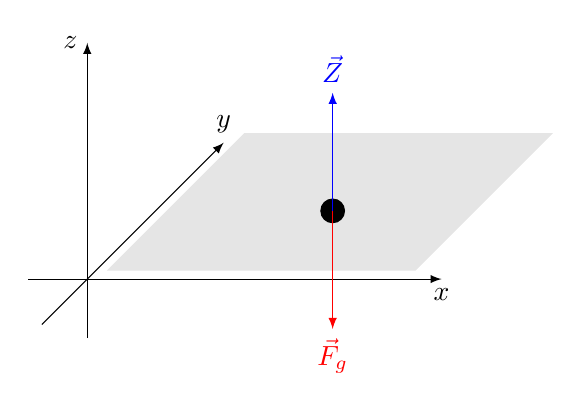
\begin{tikzpicture}[scale=1.5]
  \draw[fill,gray] (xyz cs:x=0.1,z=-0.2) -- ++(xyz cs:x=2.6) -- ++(xyz cs:z=-3) -- ++(xyz cs:x=-2.6) -- cycle;
  \draw[->] (xyz cs:x=-0.5) -- (xyz cs:x=3) node[below] {$x$};
  \draw[->] (xyz cs:y=-0.5) -- (xyz cs:y=2) node[left] {$z$};
  \draw[->] (xyz cs:z=1) -- (xyz cs:z=-3) node[above] {$y$};
  \draw[fill,black] (xyz cs:x=1.5,z=-1.5) circle (0.1);
  \draw[->,red] (xyz cs:x=1.5,z=-1.5) -- ++(0,-1) node[below] {$\F_g$};
  \draw[->,blue] (xyz cs:x=1.5,z=-1.5) -- ++(0,+1) node[above] {$\Z$};
\end{tikzpicture}
\end{document}
